\documentclass[12pt]{exam}
\usepackage{amsthm}
\usepackage{bm}
\usepackage{libertine}
\usepackage[utf8]{inputenc}
\usepackage[margin=0.5in]{geometry}
\usepackage{amsmath,amssymb}
\usepackage{multicol}
\usepackage[shortlabels]{enumitem}
\usepackage{siunitx}
\usepackage{physics}
\usepackage{booktabs}
\usepackage{graphicx}
\usepackage{pgfplots}
\usepackage{listings}
\usepackage{tikz}
\usepackage{tikz-3dplot}

\bmdefine{\ii}{i}                       %% cuaternion i
\bmdefine{\jj}{j}                       %% cuaternion j
\bmdefine{\kk}{k}                       %% cuaternion k
\newcommand{\te}{\theta}                %% short for  \theta
\newcommand{\cC}{\mathcal{C}}

\newcommand{\word}[1]{\quad\text{#1}\quad} %% texto intercalado


\pgfplotsset{width=10cm,compat=1.9}
\usepgfplotslibrary{external}
\tikzexternalize

\newcommand{\class}{Math 261-001} % This is the name of the course 
\newcommand{\examnum}{Quiz 6} % This is the name of the assignment
\newcommand{\examdate}{October 10} % This is the due date





\begin{document}
\pagestyle{plain}
\thispagestyle{empty}

\noindent
\textbf{\class}\\
\textbf{\examnum}, \textbf{\examdate} \\

% Name \hfill CSU ID \# \hspace{2.25in}

%\vspace{10 pt}

\setlength{\tabcolsep}{3.5cm} % Default value: 6pt
\renewcommand{\arraystretch}{1.5}
\setlength\extrarowheight{1cm}
\begin{tabular}{ |c|c| } 
 \hline
 Name   & CSU ID \#  \\ 
 \hline
\end{tabular}
% ---
\vspace{10pt}
\iffalse

    \foreach \s in {1,...,5}{
          \choice $P_\s$ has no power 
     }%;
\fi

Be sure to read each question carefully. You must choose and answer \textbf{exactly two} of the four problems.  
If you attempt more than two, only the first two will be graded.  
Write your final answers in the boxes provided. Each problem is worth the same amount of points.  
\textbf{Each problem is accompanied by a figure to help you visualize the region in question.}  


\begin{enumerate} 

\item Let $\cC$ be the curve which is the portion of the \textbf{astroid}
$$\left(\frac{x}{4}\right)^{\frac23}+\left(\frac{y}{2}\right)^{\frac23}=1$$
on the first quadrant of the plane. This curve admits the parametrization
$$r(t)=(4\cos^3(t),2\sin^3(t)),\quad 0\leq t\leq \pi/2.$$
Consider the vector field $F(x,y)=(y\cos(xy)-1,1+x\cos(xy))$ and evaluate the line integral $\int_{\cC}F\cdot\dd\vec{x}$. [Suggestion: First verify if the vector field $F$ is conservative.]
\begin{flushleft}
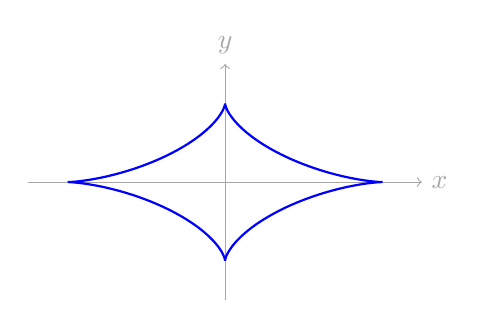
\begin{tikzpicture}[scale=0.5]
    % axes (optional)
    \draw[->,gray!70] (-5,0) -- (5,0) node[right] {$x$};
    \draw[->,gray!70] (0,-3) -- (0,3) node[above] {$y$};

    % parametric curve (x = 4cos^3 t, y = 2sin^3 t)
    \draw[thick,blue,samples=200,domain=0:360,smooth,variable=\t]
        plot ({4*cos(\t)^3}, {2*sin(\t)^3});
\end{tikzpicture}
\end{flushleft}
\begin{flushright}
\framebox(320,50){}
\end{flushright}

\item Ahhh, it's the refreshing sea breeze on your boat. Ahhh, and look! Out there is a shark eating fish, with your supreme math skills you picture the path the shark follows to be $y=x(1-x^2)$ from the points $(-1,0)$ to $(1,0)$. Also, you realize there's more fish the further away you go, so that the fish density is $f(x)=2^x$. Write down a path integral which describes the amount of fish eaten by the shark.
\begin{flushleft}
\begin{tikzpicture}[scale=1.66]
    % axes (optional)
    \draw[->,gray!70] (-1.5,0) -- (1.5,0) node[right] {$x$};
    \draw[->,gray!70] (0,-1) -- (0,1) node[above] {$y$};

    % curve (x = t, y = t(1 - t^2))
    \draw[thick,blue,samples=200,domain=-1:1,smooth,variable=\t]
        plot ({\t}, {\t*(1 - \t*\t)});
\end{tikzpicture}
\end{flushleft}
\begin{flushright}
\framebox(320,50){}
\end{flushright}

\newpage

\item Some doorstops are triangular prisms, and some have the shape of a circular section with a wedge. The doorstop you're now thinking about can ideally be described as the volume enclosed by surfaces:
$$x^2+y^2=4,\quad x=y,\quad -x=y,\quad z=0,\word{and}z=x+y.$$
Using cylindrical coordinates, write an integral representing the mass of the doorstop assuming its density is $\delta(x,y)=e^{-x^2-y^2}$. (This is, it's more massive at the tip than outside).
\begin{flushleft}
   % Set up view direction (1, -1, 1)
\tdplotsetmaincoords{75}{23}

\begin{tikzpicture}[tdplot_main_coords,scale=1.5]

% Axes
\draw[->,gray!70] (0,0,0) -- (2,0,0) node[below right] {$x$};
\draw[->,gray!70] (0,0,0) -- (0,2.5,0) node[below left] {$y$};

% Parameters
\def\r{2}

% parameters for sampling
\def\dr{0.25}   % radial step
\def\dt{5}      % angular step (degrees)
% number of radial steps: 0,0.25,...,1.75 (i=0..7) and r2 = r1+dr up to 2.0
% angular steps: j=0..17 -> t from 45 to 45+17*5 = 130, tB = tA+5 up to 135

% --- Plane patch: z = r*sin(t) (draw as small quads) ---
\foreach \j in {0,...,17} {
  \pgfmathsetmacro{\tA}{45 + \j*\dt}      % degrees
  \pgfmathsetmacro{\tB}{\tA + \dt}
  \foreach \i in {0,...,7} {
    \pgfmathsetmacro{\rA}{\i*\dr}
    \pgfmathsetmacro{\rB}{\rA + \dr}
    % four corner points (rA,tA), (rB,tA), (rB,tB), (rA,tB)
    \pgfmathsetmacro{\xA}{\rA*cos(\tA)}
    \pgfmathsetmacro{\yA}{\rA*sin(\tA)}
    \pgfmathsetmacro{\zA}{\rA*sin(\tA)}
    \pgfmathsetmacro{\xB}{\rB*cos(\tA)}
    \pgfmathsetmacro{\yB}{\rB*sin(\tA)}
    \pgfmathsetmacro{\zB}{\rB*sin(\tA)}
    \pgfmathsetmacro{\xC}{\rB*cos(\tB)}
    \pgfmathsetmacro{\yC}{\rB*sin(\tB)}
    \pgfmathsetmacro{\zC}{\rB*sin(\tB)}
    \pgfmathsetmacro{\xD}{\rA*cos(\tB)}
    \pgfmathsetmacro{\yD}{\rA*sin(\tB)}
    \pgfmathsetmacro{\zD}{\rA*sin(\tB)}
    \draw[fill=blue!32,draw=none,opacity=0.75]
      (\xA,\yA,\zA) -- (\xB,\yB,\zB) -- (\xC,\yC,\zC) -- (\xD,\yD,\zD) -- cycle;
  }
}

% --- Cylinder wall: r = 2, z from 0 to 2*sin(t) (draw as vertical quads) ---
\foreach \j in {0,...,17} {
  \pgfmathsetmacro{\tA}{45 + \j*\dt}
  \pgfmathsetmacro{\tB}{\tA + \dt}
  \pgfmathsetmacro{\xA}{2*cos(\tA)}
  \pgfmathsetmacro{\yA}{2*sin(\tA)}
  \pgfmathsetmacro{\zA}{2*sin(\tA)}   % top z at tA
  \pgfmathsetmacro{\xB}{2*cos(\tB)}
  \pgfmathsetmacro{\yB}{2*sin(\tB)}
  \pgfmathsetmacro{\zB}{2*sin(\tB)}   % top z at tB
  \draw[fill=blue!32,draw=none,opacity=0.6]
    (\xA,\yA,0) -- (\xB,\yB,0) -- (\xB,\yB,\zB) -- (\xA,\yA,\zA) -- cycle;
}

% --- Plane z = y (portion of wedge) ---

\begin{scope}
\foreach \t in {45,135} {
    \pgfmathsetmacro{\xa}{\r*cos(\t)}
    \pgfmathsetmacro{\ya}{\r*sin(\t)}
    \pgfmathsetmacro{\za}{\ya}
    \draw[fill=blue!20,draw=blue!40,opacity=0.6]
        (0,0,0) -- (\xa,\ya,0) -- (\xa,\ya,\za) -- (0,0,0);
}
\draw[fill=blue!20,draw=blue!40,opacity=0.6]
        (0,0,0) -- (\r*cos(45),\r*sin(45),\r*sin(45)) -- (\r*cos(135),\r*sin(135),\r*sin(135)) -- (0,0,0);
\end{scope}

% Cylinder boundary (circle)
\draw[dashed,gray!70,variable=\t,samples=100,domain=45:135]
    plot ({\r*cos(\t)},{\r*sin(\t)},0);

% Planes y=x and y=-x projected on xy plane
\draw[thick,gray!60] (0,0,0) -- (1.41,1.41,0) node[right,black] {$y=x$};
\draw[thick,gray!60] (0,0,0) -- (-1.41,1.41,0) node[left,black] {$y=-x$};

% Upper rim of the surface intersection with cylinder
\draw[thick,blue!80,variable=\t,samples=100,domain=45:135]
    plot ({\r*cos(\t)},{\r*sin(\t)},{\r*sin(\t)});

\end{tikzpicture}
\end{flushleft}
\begin{flushright}
\framebox(300,50){}
\end{flushright}

\item You're in one of those fancy places which serve soup in a bread bowl. Before the soup eventually breaks through the bowl and makes a mess, you decide to calculate the mass of the soup inside. Assume the soup is densest around the center, 
$$\delta(x,y,z)=\frac{1}{(x^2+y^2+z^2)^2},\quad\text{(ignore the discontinuity at the origin)}.$$
If the bowl is shaped like the sphere $x^2+y^2+z^2=1$ and has a circular opening at the plane $z=1/\sqrt{2}$ so that the bowl is everything below the plane, how much (mass of) soup does the bread bowl hold? Calculate you answer using a triple integral with spherical coordinates.
\begin{flushleft}
  \tdplotsetmaincoords{70}{110} % View direction: adjust if desired

\begin{tikzpicture}[tdplot_main_coords,scale=2]

% Axes
%\draw[->,gray!60] (0,0,0) -- (1.5,0,0) node[below right] {$x$};
%\draw[->,gray!60] (0,0,0) -- (0,1.5,0) node[below left] {$y$};
\draw[->,gray!60] (0,0,0) -- (0,0,1.5) node[above] {$z$};

% Parameters
\def\rmax{1}
\def\pmin{-90}  % -pi/2
\def\pmax{45}   % pi/4

% Sphere surface (cutoff at phi = pi/4)
\foreach \p in {-90,-75,...,30} {
  \pgfmathsetmacro\pnext{\p+15}
  \foreach \t in {0,15,...,345} {
    \pgfmathsetmacro\tnext{\t+15}
    % Current ring
    \pgfmathsetmacro\x{cos(\t)*cos(\p)}
    \pgfmathsetmacro\y{sin(\t)*cos(\p)}
    \pgfmathsetmacro\z{sin(\p)}
    % Next in phi
    \pgfmathsetmacro\xp{cos(\t)*cos(\pnext)}
    \pgfmathsetmacro\yp{sin(\t)*cos(\pnext)}
    \pgfmathsetmacro\zp{sin(\pnext)}
    % Next in theta
    \pgfmathsetmacro\xn{cos(\tnext)*cos(\p)}
    \pgfmathsetmacro\yn{sin(\tnext)*cos(\p)}
    \pgfmathsetmacro\zn{sin(\p)}
    % Corner 4
    \pgfmathsetmacro\xnp{cos(\tnext)*cos(\pnext)}
    \pgfmathsetmacro\ynp{sin(\tnext)*cos(\pnext)}
    \pgfmathsetmacro\znp{sin(\pnext)}
    % Draw patch
    \filldraw[fill=blue!20,draw=blue!40,opacity=0.6]
      (\x,\y,\z) -- (\xp,\yp,\zp) -- (\xnp,\ynp,\znp) -- (\xn,\yn,\zn) -- cycle;
  }
}

% Circle where z = 1/sqrt(2)
\def\zcap{0.7071}
\def\rcap{sqrt(1-\zcap*\zcap)}
\draw[thick,red,variable=\t,samples=100,domain=0:360]
  plot ({\rcap*cos(\t)},{\rcap*sin(\t)},{\zcap});
\node[red,right] at (0.75,0,\zcap-0.25) {$z=\tfrac{1}{\sqrt{2}}$};

\end{tikzpicture}
\end{flushleft}
\begin{flushright}
\framebox(280,50){}
\end{flushright}
\end{enumerate}

\end{document}

